\scanpage{30}\mspage{29}
% @ top, proposition heading
\uline{Proposition} Soient $F',F,G$ trois figures.
% @ top, three implications
\[
\begin{aligned}
 \text{a)}\quad F'\ll F&\Longrightarrow F'.G\ll F.G\\
 \text{b)}\quad F'\preceq F&\Longrightarrow F'.G\preceq F.G\\
 \text{c)}\quad F'\leq F&\Longrightarrow F'.G\leq F.G\quad{}^{*}
\end{aligned}
\]
% @ upper right, beside a
\margin{(trivial par déf. de $\ll$ comme Inf)}
% @ upper right, beside b
\margin{(\unsure{résulte} de a), en regardant supports)}
% @ upper left, starred gloss
\margin{$*$ \uline{\unsure{explicitation|explication}}}
% @ upper part, starred formula
\[
 F'.G=\{A\in F.G\mid A\subset |F'|\}
\]

% @ upper part, proof lines 1–2
Prouvons c. Il faut prouver que \deleted{$F'.G$} $F'.G\subset F.G$, et est fermé dans $F.G$.

% @ middle, proof lines 1–5
\deleted{\unsure{or|ces|ce}} Or $F'.G$ est formé des $A\cap B$ $(A\in F',B\in G)$ tels que $A^\circ\cap B^\circ\ne\phi$, et $F.G$ des $A\cap B$ $(A\in F,B\in \unsure{G|L})$ tels que $A^\circ\cap B^\circ\ne\phi$, et dans les deux cas \unsure{le|les} sens de $A^\circ$ (p.r. à $F$, \unsure{dans|ds} $F'$) est le $=$, donc $F'.G\subset F.G$. Prouvons que c'est fermé i.e.
% @ centre, first membership and annotations
Si \deleted{$(\deleted{A\cap B}\qquad A,A'\in F',$}
\[
 \underset{\substack{\rotatebox{-90}{$\in$}\\ F'}}{A}\cap
 \underset{\substack{\rotatebox{-90}{$\in$}\\ G}}{B}\in F'.G\qquad
 \text{i.e. } A^\circ\cap B^\circ\ne\phi
\]
% @ centre, second membership and annotations
\figure{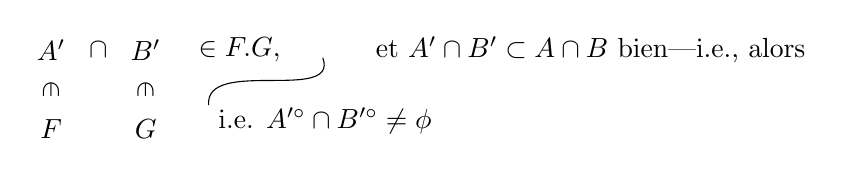
\begin{tikzpicture}[x=1cm,y=1cm]
\node at (0,0) {$A'$};
\node at (.6,0) {$\cap$};
\node at (1.2,0) {$B'$};
\node[anchor=west] at (1.75,0) {$\in F.G,$};
\node[rotate=-90] at (0,-.5) {$\in$};
\node[rotate=-90] at (1.2,-.5) {$\in$};
\node at (0,-1) {$F$};
\node at (1.2,-1) {$G$};
\node[anchor=west] at (4,0) {et $A'\cap B'\subset A\cap B$ \deleted{\unsure{bien|i.e.}}, alors};
\node[anchor=west] (ins) at (2,-.9) {\inserted{i.e. $A'^\circ\cap B'^\circ\ne\phi$}};
\draw (3.45,-.1) to[out=-70,in=95] (2,-.7);
\end{tikzpicture}}
% @ middle lower, conclusion lines 1–4
$A'\cap B'\in F'.G$ i.e. $A'\in F'$. Or on sait que (d'après la théorie de $F.G$) que $A'\cap B'\subset A\cap B\Longrightarrow A'\subset A$, $B'\subset B$, d'où $A'\in F'$ puisque $F'$ fermé dans $F$.

% @ lower left, oblique explanation
% slanted; source note rotated -45 degrees for inspection; final short label below the inverse-image line
\margin{\uline{Expliciter}~: soit
\diagram{\begin{tikzcd}[ampersand replacement=\&,column sep=small,row sep=small]
 G\arrow[r,phantom,"\leq" description]\&F\arrow[d,phantom,"\rotatebox{90}{$\unsure{\preceq|\ll}$}" description]\\
 {}\&F'
\end{tikzcd}}, d'où $G'$ \unsure{avec} $G'\preceq G$, $G'\leq F'$. Alors on a $G'=\{A'\in F'\mid A'\subset |G|\}=\varphi^{-1}(G)$, où $\varphi:F'\to F\ldots$ \unsure{$C_3$.|Cor.|C6.}}
% @ lower right, note on uniqueness; two separate vertical grouping strokes on its left are reproduced
\margin{\figure{\begin{tikzpicture}
\node[anchor=north west,inner sep=0pt,text width=2.05cm] (uppernote) at (0,0) {Un peu vif, on trouve par $F'.G=G'$ un $G'$ tel que
\diagram{\begin{tikzcd}[ampersand replacement=\&,column sep=small,row sep=small]
 F'\arrow[r,phantom,"\preceq" description] \arrow[d,phantom,"\rotatebox{90}{$\leq$}" description]\& F\arrow[d,phantom,"\rotatebox{90}{$\leq$}" description]\\
 G'\arrow[r,phantom,"\preceq" description]\& G
\end{tikzcd}}
mais il faut vérifier encore l'\uline{unicité}};
\draw ([xshift=-4pt]uppernote.north west) -- ([xshift=-4pt,yshift=1pt]uppernote.south west);
\draw ([xshift=-1pt,yshift=-7pt]uppernote.north west) -- ([xshift=-1pt,yshift=-1pt]uppernote.south west);
\end{tikzpicture}}}
% @ lower right, second note; left boundary steps right after the first b line, then descends alongside its continuation
\margin{\figure{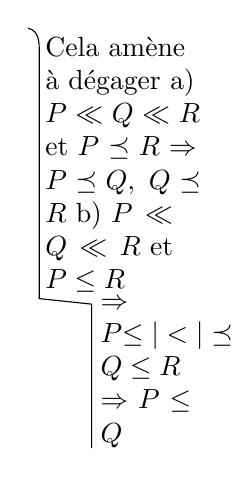
\begin{tikzpicture}
\node[anchor=north west,inner sep=0pt,text width=2.05cm] (lowernote) at (0,0) {Cela amène à dégager a) $P\ll Q\ll R$ et $P\preceq R\Rightarrow P\preceq Q,\ Q\preceq R$ b) $P\ll Q\ll R$ et $P\leq R$};
\node[anchor=north west,inner sep=0pt,text width=1.35cm] (continuation) at ([xshift=7mm,yshift=-2pt]lowernote.south west) {\deleted{$\Rightarrow P\unsure{\leq|<|\preceq}$} $Q\leq R$\\$\Rightarrow P\leq Q$};
\draw ([xshift=-6pt,yshift=3pt]lowernote.north west) .. controls ([xshift=-2pt,yshift=2pt]lowernote.north west) and ([xshift=-2pt,yshift=-2pt]lowernote.north west) .. ([xshift=-2pt,yshift=-6pt]lowernote.north west) -- ([xshift=-2pt,yshift=-2pt]lowernote.south west) -- ([xshift=-3pt,yshift=-2pt]continuation.north west) -- ([xshift=-3pt]continuation.south west);
\end{tikzpicture}}}
% @ lower part, corollary
\uline{Cor.} L'axiome C6 est valable.

% @ lower part, introduction to C7; small 0 is attached to the 7 in this main line, beside the right-note boundary
Vérifions quand même C7$_0$
% @ lower part, order diagram and existence
\diagram{\begin{tikzcd}[ampersand replacement=\&,column sep=small,row sep=small]
 G\arrow[r,phantom,"\leq" description]\arrow[d,phantom,"\rotatebox{90}{$\preceq$}" description]\&F\& {\exists\ \text{subdivision }F'\text{ de }F\text{ qui}}\\
 G'\& {}\&{\text{induise }G'.}
\end{tikzcd}}
% @ bottom, construction
On prend $F'=G'\cup\deleted{(\unsure{F\setminus G|F.G|F\times G}\unsure{2|?})}(F\setminus G)$ (réunion disjointe)
% @ bottom, verification items
Il faut vérifier a) c'est une figure b) que \deleted{\unsure{raffine}}\inserted{subdivise} $F$ et c) qui induit $G'$ sur $G$.
